	\newpage
\section{Określenie wymagań szczegółowych}		%2
\subsection{Odpowiedź na zamówienie klienta}  %1.1       

%większe wcięcie
\hspace{1cm}
\textit{
Szanowny Panie,\\
Możemy od razu zacząć realizować zamówienie, ale najpierw chciałbym omówić szczegóły techniczne. \\\\
Odniosę się do przesłanych przez Pana punktów i przedstawię rzeczy wymagające poprawy/zmiany.\\\\
1) W punkcie trzecim wspomina Pan o menu i przycisku ``Trasa''. Jeśli chodzi o poziom trudności trasy, to trzeba ustalić na jakiej podstawie ma być on wyznaczany. Moją propozycją jest tutaj stosunek przewyższenia do każdego kilometra trasy. Co do poziomu atrakcyjności dla turystów, niestety nie jest to bezpośrednio możliwe, ponieważ musielibyśmy stworzyć serwer oraz zbierać opinie i oceny od użytkowników, ale implementując Mapy Google użytkownik będzie widział ocenę miejsca którego szuka, co jest poniekąd spełnieniem Pana wymogu. \\\\
- Jeśli chodzi o przycisk ``Historia tras'' i planowanie trasy, to zamiast planowania gotowej trasy (bo przecież miejsce startu użytkownika może być różne z wielu powodów) proponuję dodać planowanie samego celu trasy. Wtedy użytkownik dostanie powiadomienie o planowanym celu i będzie mógł bezpośrednio przejść do nawigacji do określonej lokalizacji. \\\\
- Mierzenie ostrości zakrętów można poniekąd osiągnąć za pomocą akcelerometra. Wymagałoby to zbierania danych pokonując łatwe, średnie i trudne zakręty, ale będzie to trudne do uzyskania a dane i tak mogą być bardzo niedokładne. Zamiast tego proponuje dodać pomiar przeciążenia na całej trasie, co rzuci światło na oczekiwaną przez Pana ``ostrość'' trasy. \\\\
- Jeśli chodzi o pokazywanie pomiarów od 10 minut do 6 godzin wstecz, to proponuję dodać ustawienie do ilu minut/godzin wstecz pomiary mają być pokazywane, oraz przedstawiać je w formie wykresu. \\\\
2) W punkcie czwartym wspomina Pan o ekranie ładowania, który w mojej opinii nie jest potrzebny, ponieważ nie będzie interakcji ze zdalną bazą danych. Dane będą pobierane bezpośrednio z urządzenia na którym zainstalowana jest aplikacja, co będzie działo się błyskawicznie. Nie ma więc potrzeby dodawania ekranu ładowania, który będzie się wyświetlał setne części sekundy. \\\\
3) W punkcie szóstym proponuję odwrócić kolory tekstu. W jasnym motywie czarny tekst będzie kontrastowy i widoczny, a w ciemnym lepszym kolorem tekstu będzie wyróżniający się biały. Poprawi to czytelność aplikacji. \\\\
4) Jeśli chodzi o punkt dziewiąty, to niestety nie jest to możliwe do wykonania. Dokładność modułów GPS w telefonach oscyluje w granicach 5 metrów zarówno jeśli chodzi o położenie horyzontalne, jak i o wysokość urządzenia. \\\\
Pozostałe punkty na ten moment leżą w zakresie naszych możliwości. Do realizacji projektu możemy przystąpić bezzwłocznie. \\\\
Do odpowiedzi załączam zrzut ekranu zawierający proponowany wygląd ekranu głównego aplikacji, widoczny jako rysunek 2.1.\\
}

%\textit{
%Niżej przedstawiam proponowany ekran główny aplikacji:
%}

%rysunek
	\begin{figure}[!htb]
	\begin{center}
		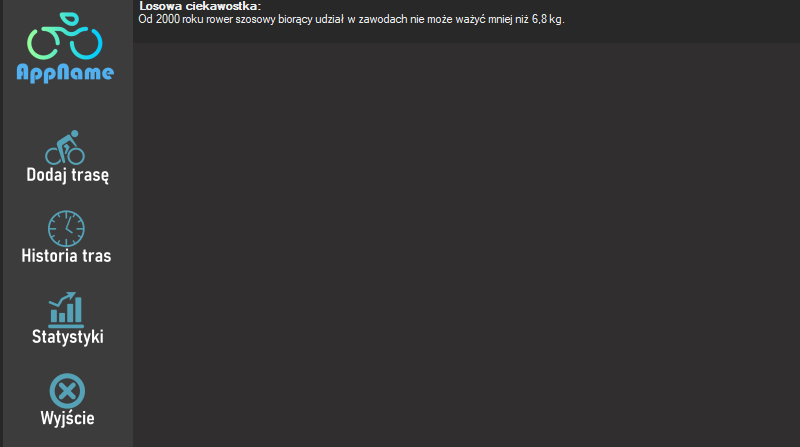
\includegraphics[width=15cm]{rys/main_screen.png}
		\caption{Propozycja ekranu głównego}
		\label{rys:Propozycja ekranu głównego}
	\end{center}
\end{figure}


